\chapter{Marco  Teórico}

En el presente capítulo se introducen conceptos fundamentales relacionados al diseño inverso de dispositivos fotónicos.
Para ello se desarrolla seis secciones. 
Primero, se describen las propiedades físicas de interés de un \emph{bend} y WDM.
Segundo, se explica como parametrizar la región de diseño de estos
dispositivos.
Tercero, se detalla los pasos necesarios para poder simular computacionalmente
los diseños realizados.
Cuarto, se explica la estrategia de optimización a seguir con la
parametrización señalada.
Quinto, se describen tres algoritmos que se usaran en el presente trabajo: (i)
algoritmos genéticos (GA), (ii) \emph{particle swarm optimization} (CMA), (iii)
\emph{covariance matrix adaptation evolution strategy}(CMA-ES).
Finalmente, se expone que transformaciones se puede aplicar dentro de la
estrategia a seguir.


\section{Dispositivos de estudio}

\subsection{\emph{Bend}}

Un \emph{bend} es un dispositivo fotónico que se encarga de guiar un haz de ondas para que gire.

En general, al estudiar dispositivos fotónicos es de especial interés la
distribución del campo eléctrico (E). 
Este campo se descompone en una componente transversal eléctrica (TE) y en una componente transversal magnética (TM) de acuerdo a la ecuación

\begin{equation}
  E = E^{TE} + E^{TM},
\label{eq:field}
\end{equation}

donde $E^{TE}$ es la componente paralela al dispositivo y $E^{TM}$ es el componente restante \citep{Hohenester2020}. 

\begin{figure}[ht]
  \centering
  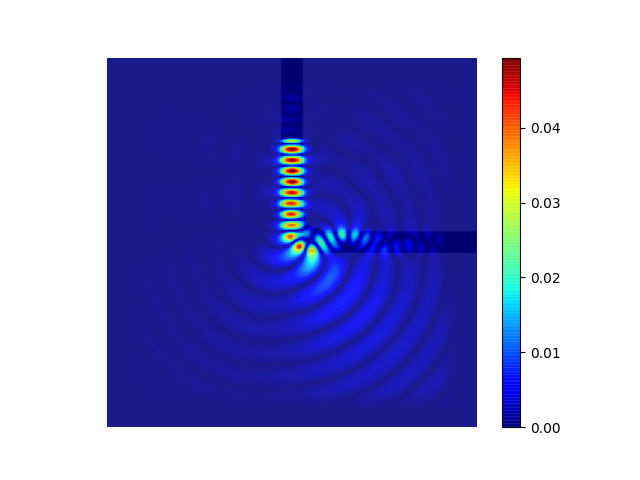
\includegraphics[scale=0.7]{image/theory/bend-field.png}
  \caption{Intensidad de campo eléctrico ($E^{TE}$) para un \emph{bend-90°} de radio interno de 0.25 $\mu m$.}
  \label{fig:efield}
\end{figure}

La intensidad de estos campos es de especial interés pues nos dan una idea del rendimiento del dispositivo. 
Por ejemplo, en la figura \ref{fig:efield} se muestra la intensidad del campo
$E^{TE}$ cuando un haz de luz está pasándo por el \emph{bend}. 
Como podemos observar, parte del campo (representando por color morado) está
fuera del dispositivo.
Así se visualiza de forma gráfica la pérdida de energía, lo cual es un indicador de mal rendimiento.

Por otro lado, para evaluar el desempeño de un dispositivo de forma numérica se
suele calcular la transmitancia ($T$) como la relación entre la intensidad del haz
que sale del dispositivo ($I$) con la intensidad con la que entra ($I_0$) \citep{Su2020}. Esto se expresa mediante la ecuación

\begin{equation}
  T = \frac{I}{I_0}.
\label{eq:transmission}
\end{equation}

Seguidamente, sea $p$ los parámetros que caracterizan a un \emph{bend}, definimos la función objetivo ($f_{obj}$) para este dispositivo,
también conocido en el área como figura de mérito (FOM), mediante la siguiente ecuación
\citep{Su2020}:

\begin{equation}
  f_{obj}(p) = max \left \{ T(p) \right \}.
\label{eq:fom-bend}
\end{equation}

Así, dentro de todas las posibles combinaciones de los parámetros $p$, la
equación $\ref{eq:fom-bend}$ busca encontrar aquellos diseños con la mayor transmitancia.
Distintas estrategias para definir los parámetros $p$ se presentan en la
\autoref{sec:parametrization} y 
los procedimientos para optimizar la función $f_{obj}$ se presentan en la
\autoref{sec:alg-opt}.

\subsection{\emph{Wavelength Demultiplexer} de dos canales (WDM)}

Un WDM es un dispositivo fotónico que se encarga de guiar un haz de ondas de acuerdo a su longitud de onda.
Así, estos suelen trabajar con dos longitudes de onda y guían las de un tipo por la guía de onda superior y las de otro tipo por la guía de onda inferior.

Similar al caso del \emph{bend} se estudia su campo eléctrico y transmitancia para medir el rendimiento de estos dispositivos.

Basándonos en \cite{Su2020}, conviene definir su FOM como

\begin{equation}
  f_{obj}(p) = max \left \{ g_0(p, 0)^2 + (1 - g_0(p, 1))^2 + g_1(p, 1)^2 + (1
  - g_1(p, 0))^2 \right \},
\label{eq:fom-splitter}
\end{equation}

donde $g_0(p, i)$ representa la transmitancia asociada a la parametrización $p$ en la guía de onda $i$ para una longitud de onda de $1400 nm$ y 
      $g_1(p, i)$ representa su análogo de $g_0(p, i)$ para una longitud de onda de $1550 nm$.

La ecuación \ref{eq:fom-splitter} busca maximizar la transmitancia por la guía de onda superior y minimizarla para la guía de onda inferior cuando se recibe una longitud de onda de $1400 nm$ y lo contrario para una longitud de onda de $1550 nm$.

Un dispositivo similar al WDM es un \emph{splitter}. Este dispositivo tiene la
misma geometría, pero lo que recibe lo trata de dividir en la misma proporción
para ambas guías de onda (superior e inferior).

\section{Parametrización}\label{sec:parametrization}

Tanto para el \emph{bend} como para el WDM se define una región de diseño
mediante ciertos parámetros que puedan mapear un gran conjunto de dispositivos a considerar.
Una de la estrategias más populares para esta tarea es usar parametrización
basada en topología, esta consiste en definir una región rectangular en forma
de matriz y variar la permitividad dentro de cada celda \citep{Molesky2018}.

\begin{figure}[h]
  \centering
  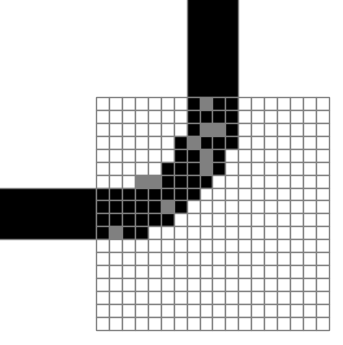
\includegraphics[scale=0.7]{image/theory/parametrization-pixeles.png}
  \caption{Parametrización por píxeles para un \emph{bend-90°.}}
  \label{fig:pixeles}
\end{figure}

Por ejemplo, en la figura \ref{fig:pixeles} se ha definido una región cuadrangular de
diseño que podemos ver como una imagen de $18 \times 18$ píxeles.
Aquí estamos usando los píxeles negros para representar la presencia de $Si$,
los blancos para indicar que hay $SiO_2$ y los grises para materiales (no
necesariamente reales) que tengan una permitividad ($\varepsilon(x, y)$) intermedia entre el $Si$
y $SiO_2$. Matemáticamente expresamos esto como

\begin{equation}
  \varepsilon(x, y) = \varepsilon_{Si} + (1 - \lambda_{x,y})
  \varepsilon_{SiO_2} \quad \lambda_{x, y} \in [0, 1], \lambda_{x, y} \in
  \mathbb{R}, 
\label{eq:permitivity}
\end{equation}

donde $\varepsilon_{Si} = 3.48$ es la permitividad del $Si$,
$\varepsilon_{SiO_2} = 1.44$ es la permitividad del $SiO2$ y $\lambda_{x, y}$
es un parámetro asociado al píxel ubicado en la fila $x$ y columna $y$.
Con esta ecuación se mapea el intervalo $[0, 1]$ con el intervalo $[1.44, 3.48]$. 
Esto se realiza para determinar la permitividad que hay en la ubicación de cada
píxel y así ser capaces de simular las ecuaciones de Maxwell en el diseño.
Con esta parametrización obtenemos una cantidad infinita de posibles dispositivos, 
mas solo nos interesan aquellos donde $\lambda_{x,y}$ es entero, 
pues en caso contrario un píxel se mapea a la permitividad de un material
potencialemente desconocido, lo cual lo volvería infabricable.

\section{Simulación}

Una vez tenemos definido un dispositivo con regiones fijas (guías de onda) y una
región de diseño (descrita por la parametrización), es necesario incorporar
tres elementos adicionales \citep{Su2020}:

\begin{itemize}

  \item \textbf{Fuente:} Suele representarse como un cuadrado en el eje $XZ$
    o $YZ$. Simula la emición de un haz de ondas por el diseño.

  \item \textbf{Monitores:} Suelen representarse como cuadrados en el eje $XZ$
    o $YZ$. Capturan información en su ubicación (e.g. valores del campo
    eléctrico).

  \item \textbf{PML:} Representan las condiciones de frontera en la simulación
    de las ecuaciones de Maxwell. Se utilizan para limitar el espacio donde se
    deberá realizar las simulaciones computacionales.

\end{itemize}

Dos librerías de Python de código abierto que permiten hacer las simulaciones
de las ecuaciones de Maxwell en diseños como los descritos son MEEP \citep{Oskooi2010} y SPINS \citep{Su2020}. 
Una evaluación cualitativa de sus funcionalidades puede ser vista en la tabla \ref{tab:simulation}.

\begin{table}[ht]
    \centering
    \begin{tabular}{|c|c|c|c|c|}
    \hline 
    Librería &  Usabilidad & Eficiencia & Bugs & Funcionalidad \\
    \hline 
    MEEP &  Difícil & Alta & Elevados & Extensa \\
    SPINS &  Moderada  & Moderada-Alta & Pocos & Básica-necesaria \\
    \hline 
    \end{tabular}
    \caption{Evaluación cualitativa de las librerías MEEP y SPINS.}
    \label{tab:simulation}
\end{table}

Ambas librerías utilizan métodos finitos para discretizar el espacio de
simulación y permiten realizar simulaciones en 2D y 3D. 
Particularmente, podemos definir un parámetro $dx$ para indicar que tan preciso
serán nuestros resultados. En general, cuanto más pequeño sea el valor de $dx$
los resultados serán más precisos, pero la cantidad de memoría y el tiempo de
simulación se incrementarán considerablemente.

Adicionalmente, hay dos diferencias importantes entre estas librerías.
Primero, en una simulación SPINS puede obtener resultados en solo una
frecuencia mientras que MEEP puede obtener resultados en un rango de
frecuencias de forma eficiente.
Segundo, MEEP realiza simulaciones en 3D utilizando MPI para aprovechar
recursos \emph{multi-cores}, por otro lado SPINS permite usar uno o más GPUs
para realizar estos cálculos.

\section{Estrategia de optimización}

Como fue descrito en la \autoref{sec:parametrization}, podemos
tener diseños que no puedan ser fabricados.
Para evitar esto se necesita obtener que $\lambda_{x, y}$ de la ecuación \ref{eq:permitivity} tenga valores enteros.
Sin embargo, al optimizar la función $f_{obj}$ no podemos asegurar esta condición.
Ante esta dificultad, \cite{Su2020} trabaja en dos etapas:


\begin{enumerate}

\item{\textbf{Optimización continua}}

En esta etapa se optimiza la función $f_{obj}$ sin imponer ninguna restricción.
    En la \autoref{sec:alg-opt} se detallará algoritmos que suelen usarse para este fin.

\item{\textbf{Optimización discreta}}

Se utiliza el resultado de la optimización continua como punto inicial para el algoritmo de optimización que se escoja.
Luego, se trabaja por iteraciones.
En cada iteración se aplica una transformación a cada diseño antes de evaluar su FOM.
Esta transformación se escoge de tal manera que asegure que una
parametrización vaya convergiendo a un diseño fabricable, es decir,
a tener $\lambda_{x, y} = 0$ o $\lambda_{x, y} = 1$, más detalles en la \autoref{sec:transformations}.
Así, la idea de realizarlo por iteraciones es para ir discretizando nuestro diseño
de forma suave e intentando mantener un buen valor del FOM.
Por ello es crucial usar el resultado de una iteración como punto inicial de la próxima

\end{enumerate}

\section{Algoritmos de optimización}\label{sec:alg-opt}

Como observamos en la anterior sección, es necesario escoger algún algoritmo
que nos permita optimizar la función $f_{obj}$. 
Por este motivo, se presentan los siguientes tres algoritmos que serán usados en el presente trabajo.

\subsection{\emph{Genetic Algorithms} (GA)}

Como se describe en el algoritmo \ref{alg:GA} \citep{Mykel2019}, la idea es  
comenzar generando una población (\emph{population}) de $n$ individuos representados por $p$
parámetros, línea 1. 
Los siguientes tres pasos se ejecutan por $k$ iteraciones.
Primero, se realiza un proceso de selección para obtener los mejores individuos
(\emph{parents}), línea 3.
Segundo, los seleccionados se encargan de producir la nueva generación
(\emph{children}), línea 4.
Tercero, la nueva generación muta obteniendo nuevas características, línea 5.

\begin{algorithm}
%\footnotesize
$population = generate\_population(n, p)$ \\
\For{$t = 0; \, t < k; \, t$++}{
    $parents = select(population)$ \\
    $children = crossover(population, parents)$ \\
    $population = mutation(children)$
}
\caption{Estructura de un algoritmo genético}
\label{alg:GA}
\end{algorithm}

Entrando en más detalle, para nuestro caso tenemos:

\begin{itemize}
    \item $generate\_population(n, p):$ retorna $n$ vectores de dimensión $p$
      con valores aleatorios en $U(0, 1)$.

    \item $select(population):$ retorna $number\_selected\_GA$ individuos de
      acuerdo a la probabilidad $prob_i$ dada por la ecuación
    
    \begin{equation}
      prob_i = \frac{f_{obj}^{(i)} - min(f_{obj})}{\displaystyle\sum_{j} (f_{obj}^{(j)} - min(f_{obj}))},
    \label{eq:prob}
    \end{equation}
    
    donde $f_{obj}^{(i)}$ está asociado con el $i-$ésimo individuo.
    
    \item $crossover(population, parents):$ retorna $n$ vectores de dimensión $p$.
    El $i-$ésimo vector es la combinación de dos padres aleatorios $pa_i$
    y $pb_i$ seleccionados de $parents$ y su $j-$ésimo parámetro es escogido
    con igual probabilidad entre el $j-$ésimo parámetro de $parents[pa_i]$
    y $parents[pb_i]$.

    \item $mutation(children):$ retorna lo que recibe, pero a cada atributo de
      cada individuo se le agrega un valor en $U(-range\_GA, range\_GA)$ con
      probabilidad de 0.5.

\end{itemize}

\subsection{\emph{Particle Swarm Optimization} (PSO)}

Podemos pensar este algoritmo como un caso especial del algoritmo \ref{alg:GA}
\citep{Mykel2019, Prosopio-Galarza2019}.
La idea es visualizar el $i-$ésimo individuo como una partícula definida por: 
(i) su posición $x^{(i)}$ (el vector $p$-dimensional asociado al $i-$ésimo individuo),
(ii) su velocidad $\nu^{(i)}$ (un número real) y
(iii) la mejor posición encontrada hasta el momento.

Cada particula acumula velocidad en una dirección favorable dada por: 
(i) la mejor posición encontrada hasta el momento por ella y 
(ii) la mejor posición encontrada por la población completa.
Como consecuencia, los individuos se pueden mover independientemente de
perturbaciones locales.
Adicionalmente, agregando caminos aleatorios las particulas incorporan
comportamientos impredecibles que puede permitirles encontrar potenciales
mejores direcciones.

Entrando en más detalle, siguiendo la estructura del algoritmo \ref{alg:GA}, tenemos:

\begin{itemize}

\item $generate\_population(n, p):$ retorna $n$ particulas con cada uno de
      sus parámetros tomando valores aleatorios en $U(0, 1)$.

\item $select(population):$ retorna la particula con el mejor $f_{obj}$

\item $crossover(population, parents):$ retorna la población luego de aplicar 
    
  \begin{equation}
    x^{(i)} \gets x^{(i)} + \nu^{(i)}
  \label{pso-pos}
  \end{equation}

  \begin{equation}
    \nu^{(i)} \gets \omega \nu^{(i)} + c_1 r_1 \left(x_{b}^{(i)} - x^{(i)}
    \right) + c_2 r_2 \left(x_{b} - x^{(i)} \right),
  \label{pso-speed}
  \end{equation}
    

  donde $x_{b}$  es la mejor posición encontrada globalmente, 
  $\omega$ representa la tendencia de la particula de conservar su velocidad actual,
  $c_1$ y $c_2$ cuantifica la atracción relativa de $x_{b}^{(i)}$ y $x_{b}$ respectivamente, 
  y $r_1, r_2 \in U(0, 1)$ representan el comportamiento impredecible.

\end{itemize}


\subsection{\emph{Covariance Matrix Adapatation Evolution Strategy} (CMA-ES)}

La idea general de esta estrategia evolutiva, mostrada en el algoritmo
\ref{alg:CMA}, es mantener:
(i) un vector $\mu$ $p$-dimensional,
(ii) una matriz $\Sigma$ y
(iii) un número $\sigma$ para ir generando $n$ inviduos $p$-dimensionales
a partir una distribución $\mathcal{N}(\mu,\,\sigma^{2} \Sigma)$.


Tomar puntos de esta distribución limita el espacio de búsqueda a una
hiperelipse.
Luego, el algoritmo evalua puntos en esta región limitada.
Usando los valores obtenidos, se puede decidir entre:
(i) mover la hiperelipse a otra región del espacio de búsqueda
(ii) expandir or reducir la región cubierta por la distribución.
El algoritmo de CMA-ES trabaja iterativamente sobre esta idea hasta que la
hiperelipse termina casi degenerándose en un punto, 
potencialmente un óptimo.
Para una descripción más detallada del algoritmo, revisar \citep{Mykel2019, Hansen2016}.

\begin{algorithm}
%\footnotesize
\For{$t = 0; \, t < k; \, t$++}{
    sample() \tcp{Obtener $n$ puntos de $\mathcal{N}(\mu,\,\sigma^{2} \Sigma)$}
    update() \tcp{Ecuación \ref{cma-average}}
    control() \tcp{Ecuación \ref{cma-control}}
    adapt() \tcp{Ecuación \ref{cma-adapt}}
}
\caption{CMA-ES}
\label{alg:CMA}
\end{algorithm}

Entrando en más detalla del algoritmo \ref{alg:CMA} y considerando variables
globales por simplicidad, podemos resumir el procedimiento en cinco pasos.
En la línea 1 simplemente se repite las siguientes líneas por $k$ iteraciones.
En la iteración $t$, comenzamos con la línea 2 generando $n$ puntos
$p$-dimensionales $x_i$ de la distribución $\mathcal{N}(\mu,\,\sigma^{2} \Sigma)$, 
donde estos son ordenados descendentemente de acuerdo
al valor de $f_{obj}$.
En la línea 3 actualizamos la media $\mu$ usando una promedio ponderado dado
por

\begin{equation}
    \mu^{(t + 1)} \gets \sum_{i=1}^{n} w_i x_i,
\label{cma-average}
\end{equation},

donde $w_i$ son fijos y escogidos de tal manera que proporcionen mayor
contribución a los puntos con meyor $f_{obj}$. Esto permite mover la media $\mu$
en una dirección favorable.

Seguidamente, se necesita actualizar $\sigma$ para expandir o reducir la
hiperelipse en la siguiente iteración. Por este motivo, la línea 4 controla
este valor mediante las ecuaciones

\begin{equation}
    \sigma^{(t + 1)} \gets \sigma^{(t)} \exp\bigg(\frac{c_{\sigma}}{d_{\sigma}}
    \underbrace{\left(\frac{||p_{\sigma}||}{\mathbb{E}||\mathcal{N}(0,
    \mathbf{I})||} - 1 \right)}_{\text{evolution path comparison}} \bigg),
\label{cma-control}
\end{equation}

\begin{equation}
\mathbb{E}||\mathcal{N}(0, \mathbf{I})|| = \sqrt{2} \left(
  \frac{\Gamma\left(\frac{p + 1}{2}\right)}{\Gamma\left({\frac{p}{2}}\right)}
  \right),
\label{cma-E}
\end{equation}

donde $p_{\sigma}$ es una variable que acumula los pasos llevados,
$c_{\sigma} \in [0, 1]$ es una variable que determina el tiempo acumulado para $p_{\sigma}$ y 
$d_{\sigma} \approx 1$ es un parámetro que determina el ratio de posibilidad de cambio de $\sigma^{(t + 1)}$. 
La principal parte de la ecuación \ref{cma-control} es el término \emph{evolution path comparison}, 
aquí se compara el tamaño de $p_{\sigma}$ con su tamaño esperado bajo selección
aleatoria.
De esta comparación podemos controlar si el valor de $\sigma$ debe
incrementarse, disminuirse o permanecer igual.

Finalmente, en la línea 5 cambiamos $\Sigma$ a una dirección favorable usando

\begin{multline}
    \Sigma^{(t + 1)} \gets \overbrace{\bigg(1 - c_1 c_c (1 - h_{\sigma})(2 - c_c) - c_1 - c_{\mu}\bigg) \Sigma^{(t)}}^{\text{cumulative update}} \\
    + \underbrace{c_{1} p_{\Sigma} p_{\Sigma}^{T}}_{\text{rank-one update}}
    + \underbrace{c_{\mu}\sum_{i=1}^{n}w'_{i}
    \delta^{(i)}\left(\delta^{(i)}\right)^{T}}_{\text{rank-}\mu\text{ update}},
\label{cma-adapt}
\end{multline}

donde $c_{\mu} \leq 1$ es el radio de aprendizaje para el término \emph{rank-$\mu$ update}, 
$c_1 \leq 1 - c_{\mu}$ es el radio de aprendizaje para el término \emph{rank-one update}, 
$c_c \in [0, 1]$ es el radio de aprendizaje para el término \emph{cumulative update}, 
$h_{\sigma}$ es la evaluación bajo la función unitaria usado para actualizar
apropiadamente el camino evolutivo, 
$p_{\Sigma}$ es un vector acumulativo usado para actualizar la matriz de
covarianza, 
$w'_i$ son los coeficientes de ponderación modificados y
$\delta^{(i)}$ son las desviaciones seleccionadas.

En la ecuación \ref{cma-adapt}, el primer término (\emph{cumulative update}) 
mantiene información de la anterior matriz de convarianza.
El segundo término (\emph{rank-one update}) permite expandir la distribución en
una dirección favorable.
El tercer término (\emph{rank-$\mu$ update}) incrementa la búsqueda en espacios
donde es probable encontrar buenas soluciones.
La combinación de estos tres términos actualiza $\Sigma$ de tal manera que
mueva la hiperelipse en una dirección favorable.

\section{Transformaciones}\label{sec:transformations}

La aplicación de transformaciones a un diseño se realiza con el fin de obtener
dispositivos que se puedan fabricar con mayor facilidad \citep{Su2020}. 

Basándonos en \cite{Zhang2021}, una manera de asegurar que los
parámetros $p$ describan un diseño más fácil de fabricar es aplicacando la función $s(p)$
descrita como

\begin{equation}
  s(p) = \frac{\tanh (\beta \times \eta) + \tanh (\beta \times (p
  - \eta))}{\tanh (\beta \times \eta) + \tanh (\beta \times (1 - \eta))},
  \label{eq:topo-smooth}
\end{equation}

    donde $\eta = 0.5$ y $\beta$ comienza con un valor de 1 y va incrementándose exponencialmente en cada iteración. 
    Como se observa en la figura \ref{fig:discretization}, la ecuación \ref{eq:topo-smooth} se encarga de ir haciendo converger los valores de la parametrización a $0$ o $1$ de acuerdo a cual esté más cercano. 
    Conforme aumenta el valor de $\beta$ esta convergencia es más rápida.

    \begin{figure}[ht]
      \centering
      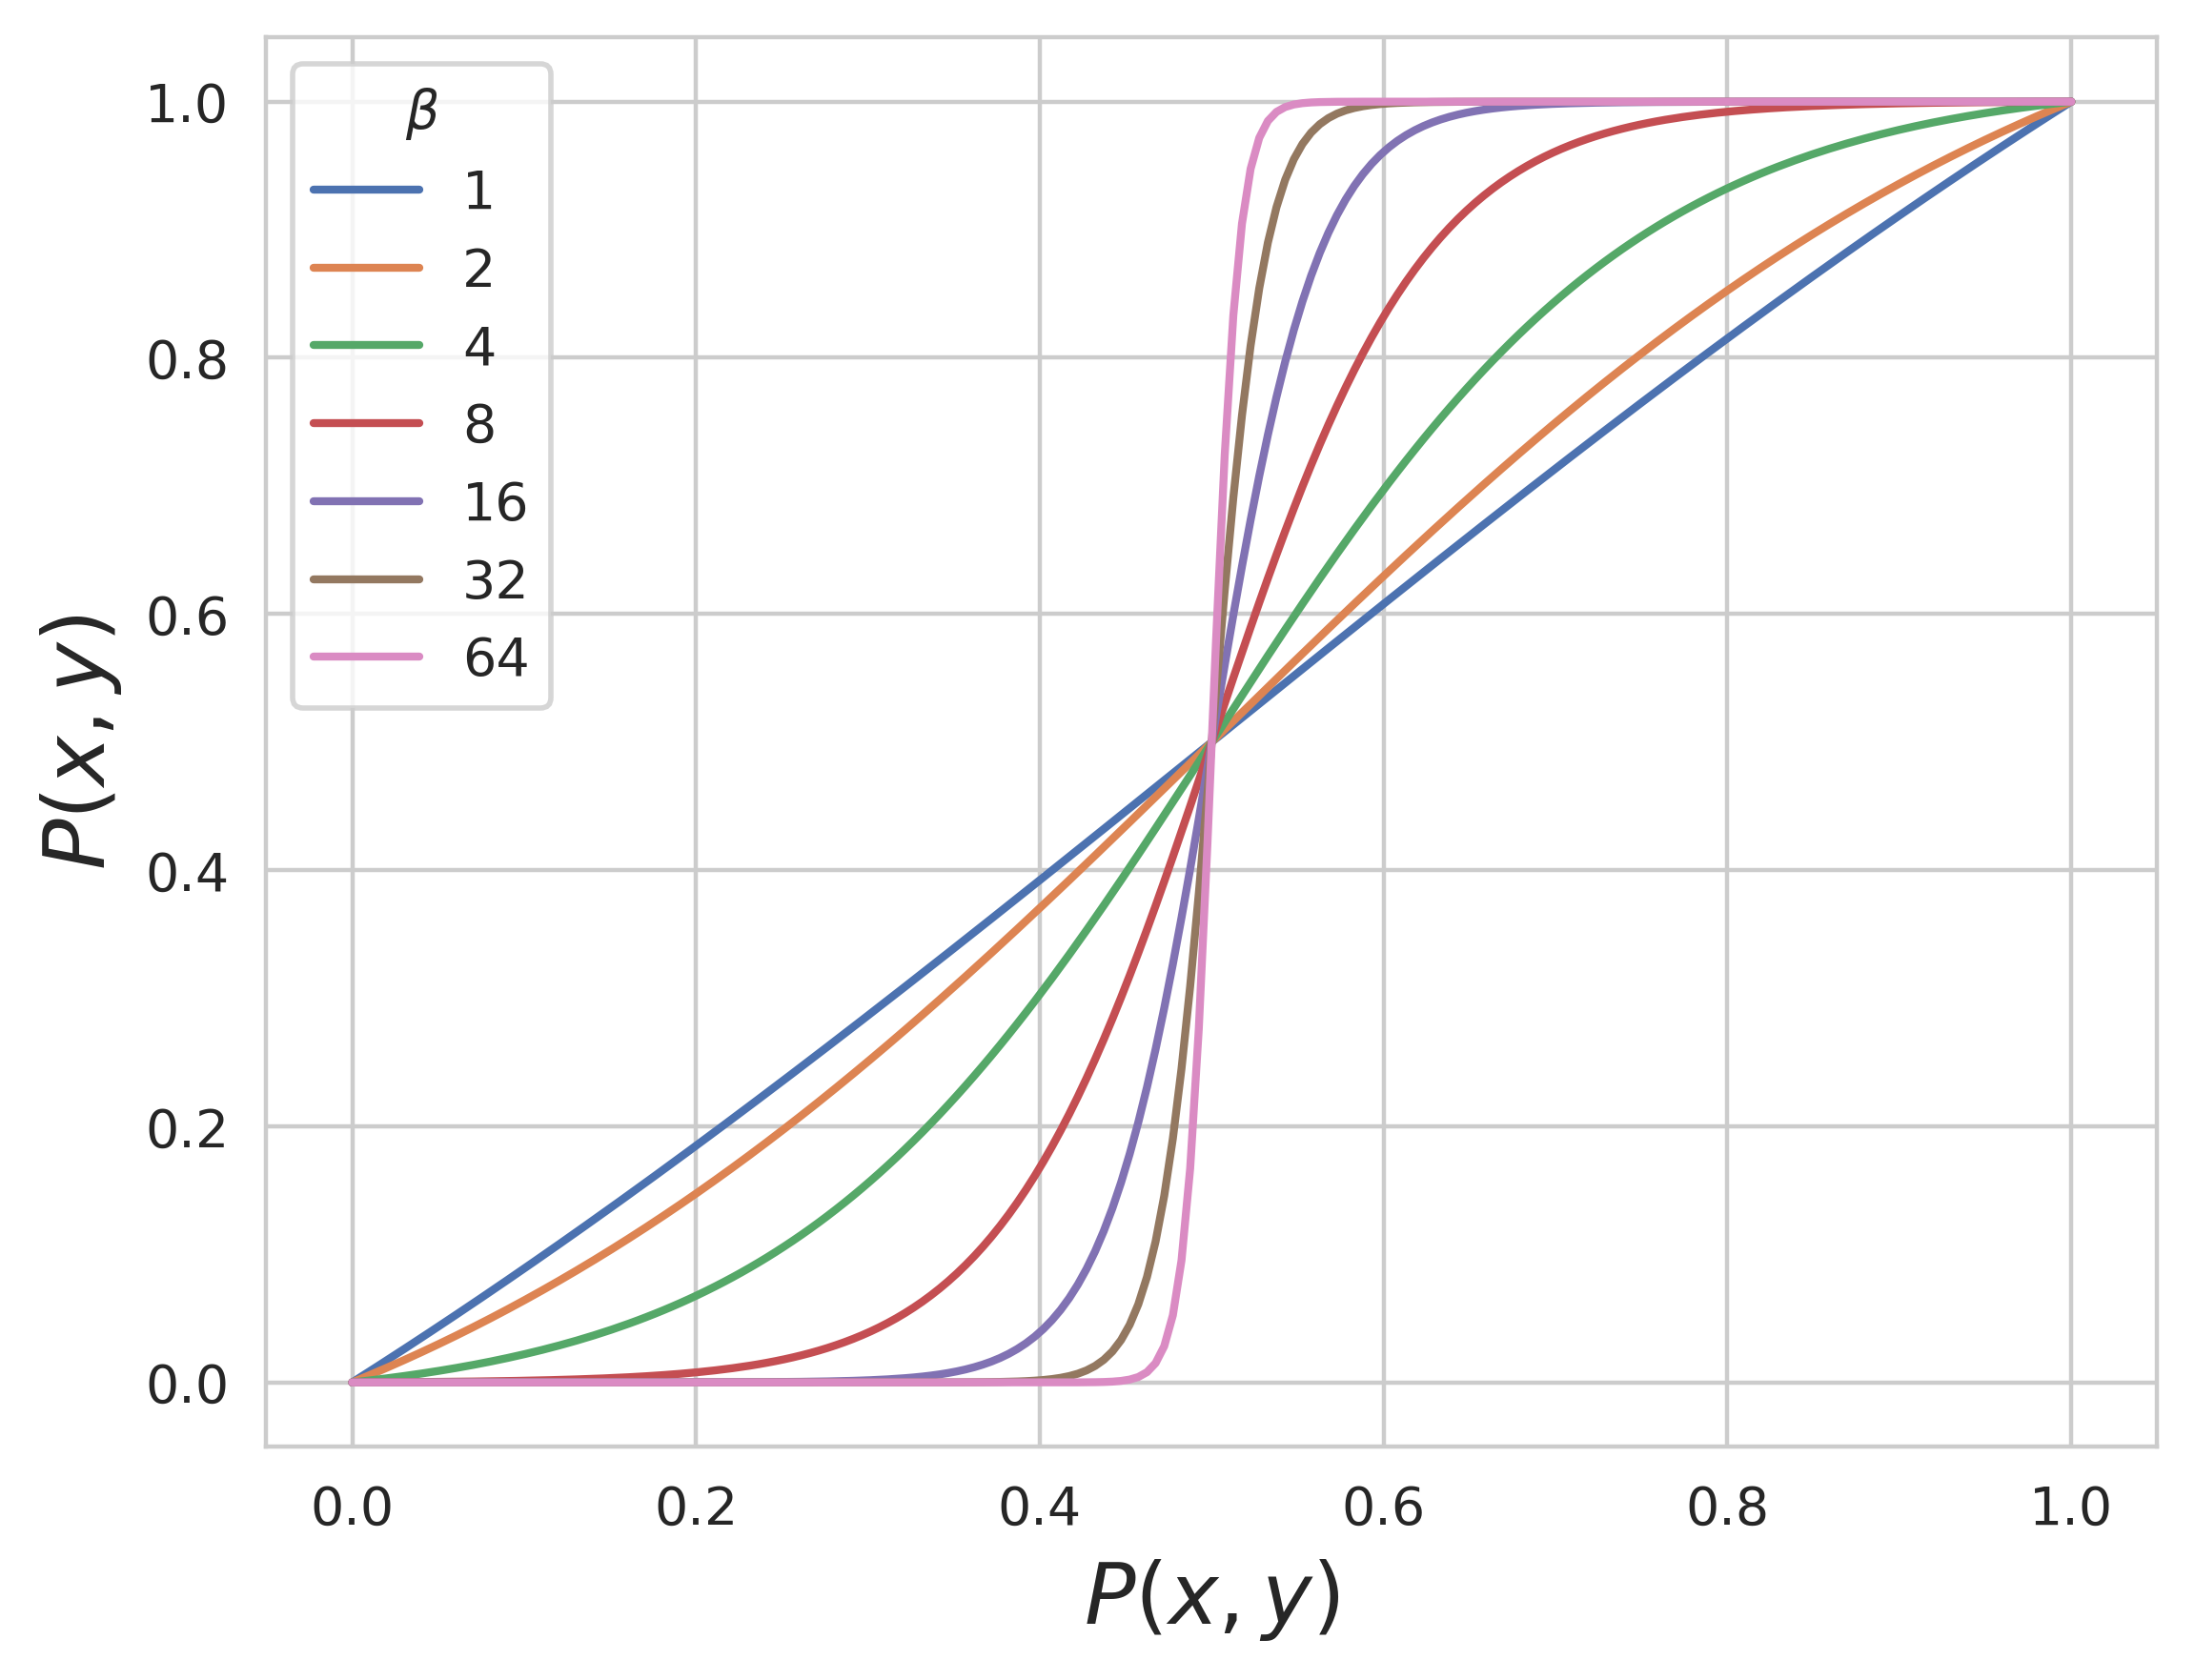
\includegraphics[scale=0.8]{image/theory/discretization.png}
      \caption{Función de discretización con $\eta = 0.5$ y distintos valores
      de $\beta$.}
      \label{fig:discretization}
    \end{figure}

%\section{Preparación para fabricación}

%\subsection{Formato GDSII}

%Para poder fabricar nuestros diseños necesitamos representarlos en formato GDSII.
%En este formato se especifica los polígonos que representan a nuestro dispositivo.
%Independientemente de la parametrización utilizada, mediante la simulación con SPINS o MEEP se puede obtener los puntos asociados al contorno del dispositivo.
%Así, utilizando lo anterior se construye los polígonos \citep{Bogaerts2018}.

%\leonidas{Hablar en más detalle de esto y acompañarlo con una imagen de conversión de una curva al formato GDSII similar al paper de Lukas}

%\subsection{Simulación de errores}

%\leonidas{Escribir las fórmulas de dilatación y contracción de Hammond2020. Hacer un link con el método de los 9 puntos.}
